\documentclass[11pt, sans, handout]{beamer}

\usepackage[utf8]{inputenc} 
\usepackage[T1]{fontenc}
\usepackage{lmodern}
\usepackage{graphicx}
\usepackage[french]{babel}
\usepackage[many]{tcolorbox}

\newtcolorbox{RDB}[2][]{%attach boxed title to top center
               = {yshift=-8pt},
  colback      = blue!5!white,
  colframe     = blue!75!black,
  fonttitle    = \bfseries,
  colbacktitle = blue!85!black,
  title        = #2,#1,
  enhanced,
}

\usetheme{Copenhagen}

\addtobeamertemplate{footline}{\insertframenumber/\inserttotalframenumber}


\begin{document}
\title{Comparaison des modèles de base de données relationnel et en graphe}
\date{15 mai 2019}
\maketitle

\frame{
	\frametitle{Rappel théorique}
	\framesubtitle{Base de données relationnelle}
	Dans une base de données relationelle, les données sont organisées en tables. Les colonnes de ces tables sont appelées des attributs et les lignes sont appelées des tuples.\\
	\begin{center}
	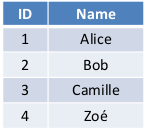
\includegraphics[scale=0.62]{resources/BDR1.png}
	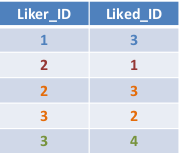
\includegraphics[scale=0.62]{resources/BDR2.png}
	\end{center}
	Les tables d'une BDR respectent des contraintes et des clés.\\
}

\frame{
	\frametitle{Rappel théorique}
	\framesubtitle{Base de données en graphe}
	Dans une base de données en graphe, les données sont contenues dans des noeuds, et les relations entre les données sont décrite par les arcs reliant ces noeuds. A chaque tupe des tables d'une BDR correspond un noeud en BDG. La base de donnée prend la forme d'un graphe orienté.
	\begin{center}
	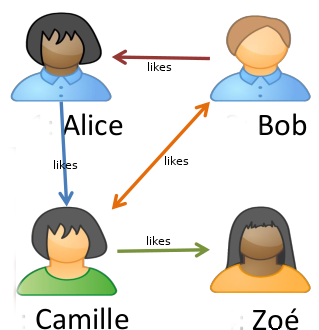
\includegraphics[scale=1.75]{resources/BDG1.png}
	\end{center}
}

\frame{
	\frametitle{Comparaison des modèles}
	\framesubtitle{Efficacité lors de la séléction}
	Maintenant que nous avons nos données stockées selon les deux modèles, effectuons une requête.
	Commencons par une requête simple :
	\emph{Qui est-ce que Bob aime ?}
}
	\frametitle{Comparaison des modèles}
	\framesubtitle{Efficacité lors de la séléction}
	
\frame{
	\frametitle{Comparaison des modèles}
	\framesubtitle{Efficacité lors de la séléction}
	Dans notre base de données relationnelle :\\
	\begin{itemize}
		\item Rechercher dans la table (ID, name) Bob, pour connaitre son ID.
		\item Rechercher dans la table (liker\_ID, liked\_ID) toutes les occurence de l'ID de Bob.
	\end{itemize}
	\begin{center}
		\includegraphics[scale=.9]{resources/reqBDR1.png}
		
	\end{center}
}

\frame{
	\frametitle{Comparaison des modèles}
	\framesubtitle{Efficacité lors de la séléction}
	Dans notre base de données en graphe :\\
	\begin{itemize}
		\item Trouver Bob.
		\item Les arcs "liked" partant de Bob nous donne immédiatement l'information recherchée.
	\end{itemize}
	\begin{center}
	\includegraphics[scale=1.25]{resources/reqBDG1.png}
	\end{center}
}

\frame{
	\frametitle{Comparaison des modèles}
	\framesubtitle{Efficacité lors de la séléction}
	Intéressons nous maintenant à une requête plus compliquée sur une autre base de données.\\
	\emph{Quel est ce film parlant de sous-marins dans lequel joue l'acteur qui était dans un autre film aux cotés de l'acteur principal de "Gone With the Wind" ?}
}

\frame{
	\frametitle{Comparaison des modèles}
	\framesubtitle{Efficacité lors de la séléction}
	Dans notre base de données relationnelle :\\
	\begin{itemize}
		\item Trouver les acteurs de "Gone With the Wind".
		\item Trouver tous les films dans lesquels ces acteurs ont joués.
		\item Trouver tous les acteurs ayant joués dans ces films et n'étant pas l'acteur principal de "Gone With the Wind".
		\item Trouver tous les films dans lesquels chacuns de ces acteurs ont joués.
		\item Finalement, rechercher le mot "sous-marin" dans la description de ceux-ci.
	\end{itemize}
}

\frame{
	\frametitle{Comparaison des modèles}
	\framesubtitle{Efficacité lors de la séléction}
	Dans notre base de données en graphe :\\
	\begin{itemize}
		\item Trouver le noeud "Gone With the Wild".
		\item Suivre le lien "a comme acteur principal" pour arriver a Clark Gable.
		\item Suivre les liens "a joué dans" en partant de celui-ci.
		\item Suivre les liens "a pour acteur" en partant des films ainsi atteints.
		\item Suivre les liens "a joué dans" en partant de ceux-ci.
		\item Examiner les noeuds atteints à la recherche du mot "sous-marin".
	\end{itemize}
	Nous n'avons fait que suivre des liens, aucune recherche n'a été effectuée.
}

\frame{
	\frametitle{Comparaison des modèles}
	\framesubtitle{Efficacité lors de la séléction}
	\begin{center}
		\includegraphics[scale=0.3]{resources/imageGDR1.png}
	\end{center}
	Exemple de la diversité d'informations contenue dans une base de données en graphe.\\[.1cm]
	\tiny Source : \emph{https://arstechnica.com/information-technology/2013/03/knowing-the-score-how-facebooks-graph-search-knows-what-you-want/?fbclid=IwAR2EOPrLyCSpvCYYVMuaAN094E6yqHGojkxAwxJCgiZAFIMZFob4NjHLM4k}
	
}

\frame{
	\frametitle{Comparaison des modèles}
	\framesubtitle{Autres avantages/inconvénients du modèle relationnel}
	\textbf{Avantages :}
	\begin{itemize}
		\item L'application d'une transformation sur un grand nombre de ligne de la table est immédiate.
		\item Le modèle est plus ancien et plus répandu. Il a donc été plus étudié et beaucoup d'outils robustes sont disponibles.
		\item L'espace de stockage requis est minimal.
	\end{itemize}
	\textbf{inconvénients :}
	\begin{itemize}
		\item Les grosses requêtes de séléction sont lourdes à exécuter.
		\item Le modèle est moins flexible, ajouter un attribut nécessite beaucoup de changements au sein des tables.
	\end{itemize}
	
	
}

\frame{
	\frametitle{Comparaison des modèles}
	\framesubtitle{Autres avantages/inconvénients du modèle en graphe}
	\textbf{Avantages :}
	\begin{itemize}
		\item L'ajout d'un attribut est immédiat, il suffit de créer des arcs supplémentaires entre les données, ou un champ de plus dans les noeuds concernés.
		\item Les requêtes de séléctions sont rapides a exécuter.
	\end{itemize}
	\textbf{inconvénients :}
	\begin{itemize}
		\item Le modèle est récent, donc il a moins été étudié et moins d'outils sont disponibles.
		\item L'espace de stockage requis est plus élevé.
	\end{itemize}
}

\frame{
	\frametitle{Conclusion}
	\framesubtitle{Dans le cas de l'utilisation d'un des deux modèles}
	\textbf{Le modèle relationnel} est adapté à une base de donnée avec peu de relation entre les donnés, ou lorsqu'il y a beaucoup d'écriture à effectuer.\\
	\textbf{Le modèle en graphe} par contre est adapté pour de grosses bases de données, régies par beaucoup de relation, ou si l'on doit effectuer beaucoup de lectures.
}

\frame{
	\frametitle{Conclusion}
	\framesubtitle{Vers une utilisation mixe des modèles}
	La solution idéale reste d'utiliser simultanément les deux modèles, par exemple :\\
	\begin{itemize}
		\item Un modèle en graphe dont les noeuds contiennent des tables du modèle relationnel.
		\item Un modèle en graphe dont les plus gros noeuds sont référencés par une table du modèle relationnel.
		\item Une base de données relationnelle pour l'écriture, correspondant à une base de données en graphe pour les lectures.
		\item ... 
	\end{itemize}
}

\frame{
	\frametitle{Fin}
	Questions ?\\[2cm]
	Merci de votre attention.
}


\end{document}